\documentclass[12pt,a4paper]{article}

\usepackage[utf8]{inputenc}
\usepackage[T1]{fontenc}
\usepackage[french]{babel}
\usepackage{lmodern}
\usepackage[a4paper,margin=2.5cm]{geometry}
\usepackage{amsmath,amssymb}
\usepackage{graphicx}
\usepackage{float}
\usepackage{hyperref}

\title{\textbf{TP3 -- Filtrage}}
\author{Fatimetou Narjah}
\date{Octobre 2026}

\begin{document}

\maketitle

\section{Introduction}

L'objectif de cette question est d'étudier l'influence
de la manoeuvre de l'observateur sur la précision du
pistage d'un émetteur à partir de mesures angulaires.
Pour cela, on utilise la borne de Cramèr-Rao (BCR),
qui permet d'évaluer la limite théorique de précision
de l'estimation. Il s'agit de calculer cette borne à
l'instant final $n$ en fonction de l'angle de manoeuvre
$\varphi$, puis d'analyser les performances associées
aux différentes trajectoires de l'observateur.


\section{Q1 -- Optimisation de la manœuvre par la borne de Cramèr-Rao}

\subsection{Q1a -- Construction du code de calcul de la BCR}

L'objectif de cette première question est d'implémenter le calcul récursif de la borne de Cramèr-Rao dans le cas d'une dynamique linéaire non bruitée et de mesures gaussiennes. Cette borne permet d'évaluer la limite théorique de précision que peut atteindre un estimateur de l'état.

On considère une cible dont l'état à l'instant $k$ est défini par :
\begin{equation}
X_k =
\begin{pmatrix}
x_k & y_k & \dot{x}_k & \dot{y}_k
\end{pmatrix}^{T}.
\end{equation}

La dynamique est supposée linéaire et déterministe, décrite par :
\begin{equation}
X_k = \Phi X_{k-1},
\end{equation}
avec :
\begin{equation}
\Phi =
\begin{pmatrix}
1 & 0 & T & 0\\
0 & 1 & 0 & T\\
0 & 0 & 1 & 0\\
0 & 0 & 0 & 1
\end{pmatrix},
\end{equation}
où $T$ représente le pas de temps entre deux mesures.

La mesure considérée est une mesure angulaire (azimut) :
\begin{equation}
Y_k = h_k(X_k)+\epsilon_k,
\end{equation}
où $\epsilon_k$ est un bruit gaussien centré de variance $\sigma_k^2$.

La matrice d'information de Fisher initiale est donnée par :
\begin{equation}
J_0=P_0^{-1},
\end{equation}
où $P_0$ représente la covariance initiale de l'état.

Pour une dynamique non bruitée, la propagation de l'information et l'ajout de la nouvelle mesure sont effectués selon la relation récursive :
\begin{equation}
\boxed{
J_k =
\Phi^{-T}J_{k-1}\Phi^{-1}
+
\frac{1}{\sigma_k^2}
H_k^T H_k
}
\end{equation}
où $H_k=\nabla_{X_k}h_k(X_k)$ est le gradient de la fonction de mesure.

La borne de Cramèr-Rao est ensuite obtenue par inversion de la matrice d'information :
\begin{equation}
\boxed{\mathrm{BCR}_k=J_k^{-1}.}
\end{equation}

Dans le cadre de ce TP, la fonction de mesure correspond à l'angle entre l'observateur et la cible :
\begin{equation}
h_k(X_k)=
\operatorname{atan2}
(y_k-y_k^o,x_k-x_k^o),
\end{equation}
où $(x_k^o,y_k^o)$ désignent les coordonnées de l'observateur.

En posant :
\begin{equation}
\Delta x_k=x_k-x_k^o,\qquad
\Delta y_k=y_k-y_k^o,
\end{equation}
la dérivée de la fonction de mesure par rapport à l'état est :
\begin{equation}
H_k =
\begin{pmatrix}
-\dfrac{\Delta y_k}{\Delta x_k^2+\Delta y_k^2}
&
\dfrac{\Delta x_k}{\Delta x_k^2+\Delta y_k^2}
&
0&0
\end{pmatrix}.
\end{equation}

Les deux dernières composantes sont nulles puisque la mesure angulaire ne dépend pas directement des vitesses de la cible.

L'implémentation Python a été réalisée dans le fichier \texttt{cramer\_rao\_deterministe.py}. Deux opérations principales ont été programmées : la propagation de la matrice d'information à travers la dynamique, puis l'ajout de l'information apportée par la nouvelle mesure.

La méthode \texttt{predict(F)} réalise la propagation :
\begin{equation}
J_k^{\mathrm{pred}}=F^{-T}J_{k-1}F^{-1},
\end{equation}
tandis que la méthode \texttt{update(H,R)} ajoute l'information de mesure :
\begin{equation}
J_k=J_k^{\mathrm{pred}}+H^TR^{-1}H.
\end{equation}

La covariance associée à la borne est ensuite calculée par inversion de la matrice d'information. Cette implémentation permet ainsi de suivre l'évolution de la précision théorique de l'estimation au cours du temps.



\subsubsection{Étude du cas particulier $\varphi=0$ sans information a priori}

On étudie tout d'abord le cas où l'observateur
ne réalise aucune manoeuvre, c'est-à-dire
$\varphi=0$. Il poursuit alors une trajectoire
rectiligne à vitesse constante.

Afin d'étudier l'observabilité du système sans
information a priori, on initialise la matrice
d'information par :

\[
J_0=0_{4\times4}.
\]

La récurrence de la matrice d'information est
ensuite appliquée en utilisant les mesures
angulaires successives.

L'analyse numérique des valeurs singulières
de la matrice d'information finale donne :

\[
s(J_n)=
\begin{pmatrix}
147.4345\\
0.06849\\
0.005350\\
2.37\times10^{-16}
\end{pmatrix}.
\]

La dernière valeur singulière étant pratiquement
nulle, on obtient :

\[
\boxed{\operatorname{rang}(J_n)=3<4}
\]

La matrice d'information finale est donc
singulière et son inverse n'existe pas.

Cette perte de rang traduit la non-observabilité
du système : lorsque l'observateur suit une
trajectoire rectiligne à vitesse constante,
plusieurs trajectoires de l'émetteur peuvent
produire les mêmes mesures angulaires.

La singularité de la matrice d'information signifie qu'il existe au moins une direction de l'espace d'état dans laquelle l'information disponible est insuffisante pour déterminer l'état. Par conséquent, la matrice \(J_n^{-1}\) ne peut pas être calculée et la BCR complète n'est pas définie par inversion classique.

Ainsi, ce résultat met en évidence l’importance de la manœuvre de l’observateur pour améliorer l’observabilité et la précision du pistage.

\subsection{Q1b -- Optimisation de l'angle de manœuvre}

Cette question consiste à déterminer le cap que doit adopter l'observateur après sa manœuvre afin de minimiser l'incertitude finale sur la position de la cible.

On considère une cible se déplaçant à vitesse constante, sans bruit dynamique, et un observateur se déplaçant initialement selon l'axe horizontal positif. Une modification instantanée de son cap est effectuée au milieu de la séquence de mesures.

Les paramètres utilisés dans la simulation sont :
\begin{itemize}
    \item Pas temporel : $T=1\,\mathrm{s}$.
    \item Nombre de mesures : $N=100$.
    \item Écart-type du bruit angulaire : $\sigma_\theta=1^\circ$.
    \item Vitesse de l'observateur : $V_o=10\,\mathrm{m/s}$.
    \item Vitesse de la cible : $V_c=5\,\mathrm{m/s}$.
    \item Cap initial de la cible : $-20^\circ$.
    \item État initial de la cible : $(2000,2000)$ en position.
    \item Covariance initiale de l’état : P₀ = diag(1000², 1000², 10², 10²).
\end{itemize}

Le cap adopté par l'observateur après la manœuvre est noté $\varphi$. Pour chaque valeur de cet angle, une nouvelle trajectoire nominale de l'observateur est construite, puis la matrice d'information de Fisher est calculée récursivement à chaque instant.

L'objectif est de minimiser la somme des bornes de variance associées aux deux coordonnées de position à l'instant final $n$. Le critère d'optimisation est donc défini par :
\begin{equation}
\boxed{
C(\varphi)=
\operatorname{tr}
\left(
\mathrm{BCR}_n(\varphi)_{1:2,1:2}
\right)
}
\end{equation}

Ce qui revient à minimiser :
\begin{equation}
C(\varphi)=
\mathrm{BCR}_{xx}(\varphi)
+
\mathrm{BCR}_{yy}(\varphi).
\end{equation}
Ce critère correspond à la somme des bornes inférieures des variances d'estimation des deux coordonnées de position. Sa minimisation permet donc de rechercher la manœuvre qui offre la meilleure précision théorique sur la position de la cible à l'instant final. La racine carrée de ce critère fournit une mesure globale de l'incertitude de position en mètres.

La valeur optimale recherchée est :
\begin{equation}
\boxed{
\varphi_{\mathrm{opt}}
=
\arg\min_{\varphi\in[0,360[} C(\varphi).
}
\end{equation}

Le programme \texttt{q1\_manoeuvre.py} réalise cette recherche par balayage d'une grille d'angles. Le paramètre \texttt{--step-deg} permet de définir le pas de discrétisation de cette grille. Une première exécution a été effectuée avec un pas de $0.1^\circ$, puis une seconde avec un pas plus fin de $0.01^\circ$ afin de vérifier la stabilité du résultat.

La précision finale est également exprimée par la racine carrée du critère :
\begin{equation}
\mathrm{RMS}_{2D}(\varphi)=\sqrt{C(\varphi)}.
\end{equation}

\paragraph{Résultats et interprétation}

La première simulation, réalisée avec un pas de $0.1^\circ$, donne un angle optimal de $115^\circ$. Le critère minimal obtenu est de $13349.589\,\mathrm{m}^2$, correspondant à une RMS de $115.540\,\mathrm{m}$.

En affinant le pas de recherche à $0.01^\circ$, l'angle optimal obtenu est de $114.9^\circ$, avec un critère minimal de $13349.546\,\mathrm{m}^2$ et une RMS de $115.540\,\mathrm{m}$.

Les deux résultats étant très proches, cette comparaison confirme la stabilité numérique de l'optimum obtenu. On retiendra donc :
\begin{equation}
\boxed{
\varphi_{\mathrm{opt}}=114.9^\circ
}
\end{equation}
et :
\begin{equation}
\boxed{
C_{\min}=13349.546\,\mathrm{m}^2,
\qquad
\mathrm{RMS}_{2D,\min}=115.540\,\mathrm{m}.
}
\end{equation}

La figure suivante présente l'évolution de la RMS finale en fonction du cap adopté après la manœuvre.

\begin{figure}[H]
    \centering
    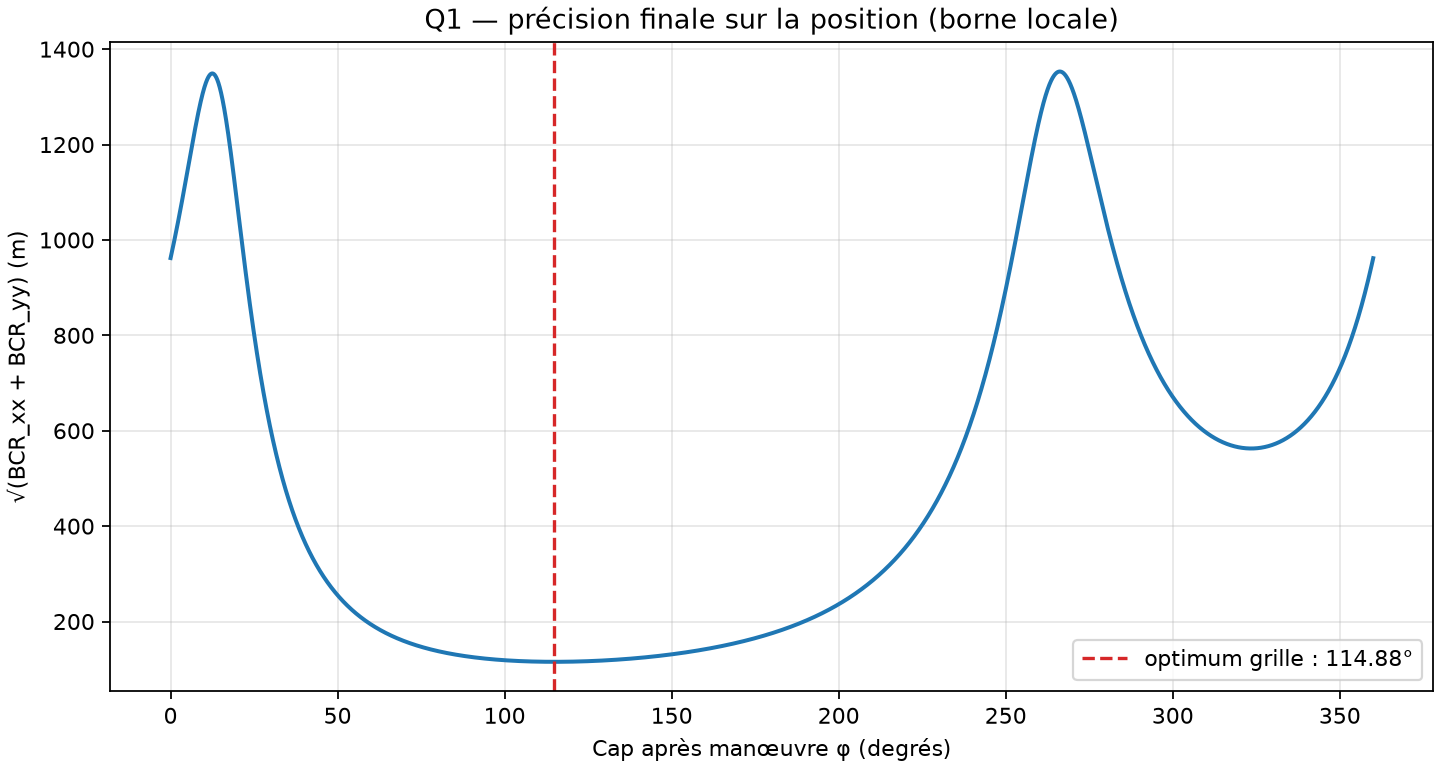
\includegraphics[width=0.65\textwidth]{q1_grille.png}
    \caption{Évolution de la RMS finale de position en fonction de l'angle de manœuvre.}
    \label{fig:q1_grille}
\end{figure}

La courbe présente un minimum principal autour de $115^\circ$, ce qui correspond à la meilleure précision finale parmi les angles testés. On observe également une autre zone de minimum autour de $325^\circ$, mais celle-ci conduit à une incertitude plus importante. Les variations de la courbe montrent que la précision du pistage dépend fortement du cap choisi par l'observateur et, par conséquent, de la géométrie relative entre celui-ci et la cible.

La deuxième figure représente les trajectoires nominales de la cible et de l'observateur pour l'angle optimal obtenu.

\begin{figure}[H]
    \centering
    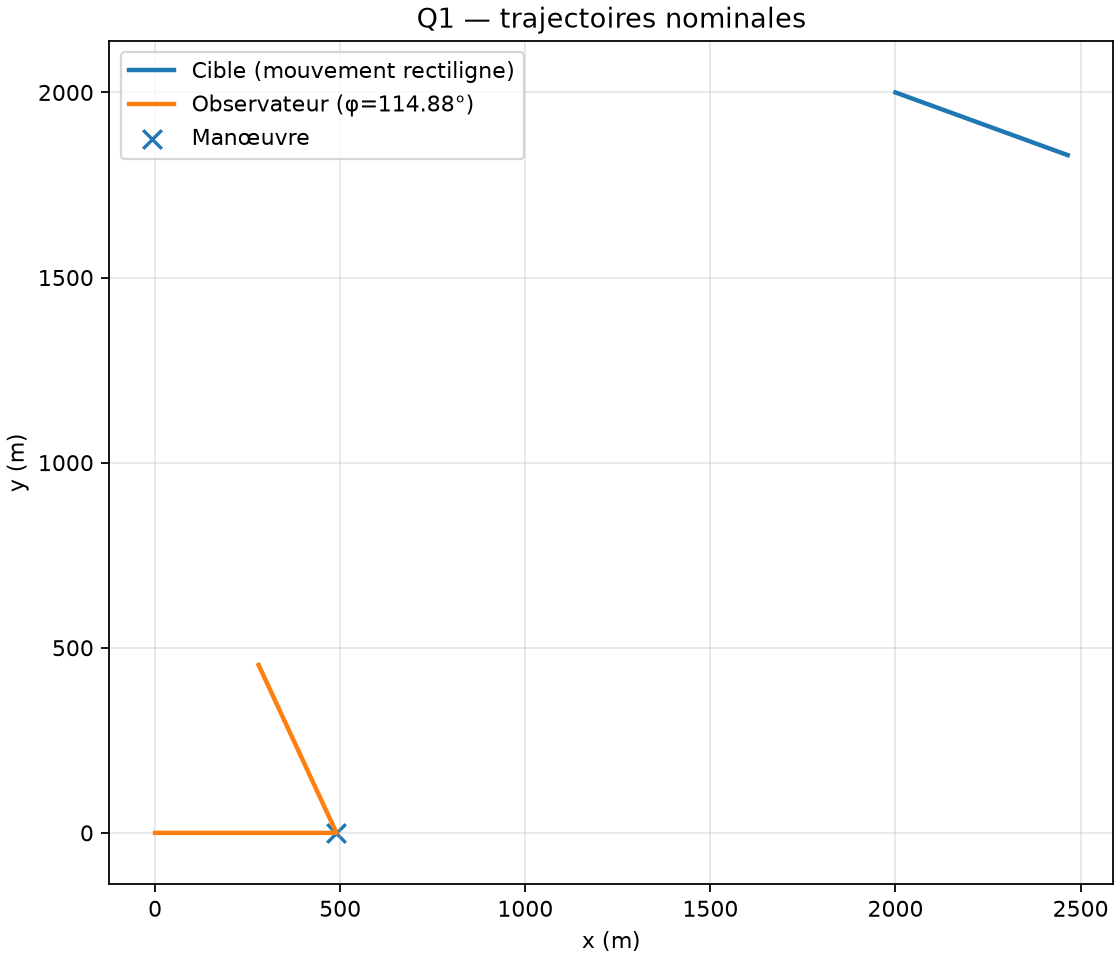
\includegraphics[width=0.5\textwidth]{q1_trajectoires.png}
    \caption{Trajectoires nominales de la cible et de l'observateur pour le cap optimal.}
    \label{fig:q1_trajectoires}
\end{figure}

La cible suit une trajectoire rectiligne à vitesse constante, tandis que l'observateur se déplace initialement selon l'axe $+x$, puis modifie son cap après la manœuvre. Le changement de direction permet de modifier la géométrie d'observation et d'améliorer les conditions de mesure angulaire. La position du point de manœuvre est également indiquée sur la figure.

Enfin, la troisième figure illustre l'évolution temporelle des écarts-types associés aux bornes de variance des composantes de position et de vitesse.

\begin{figure}[H]
    \centering
    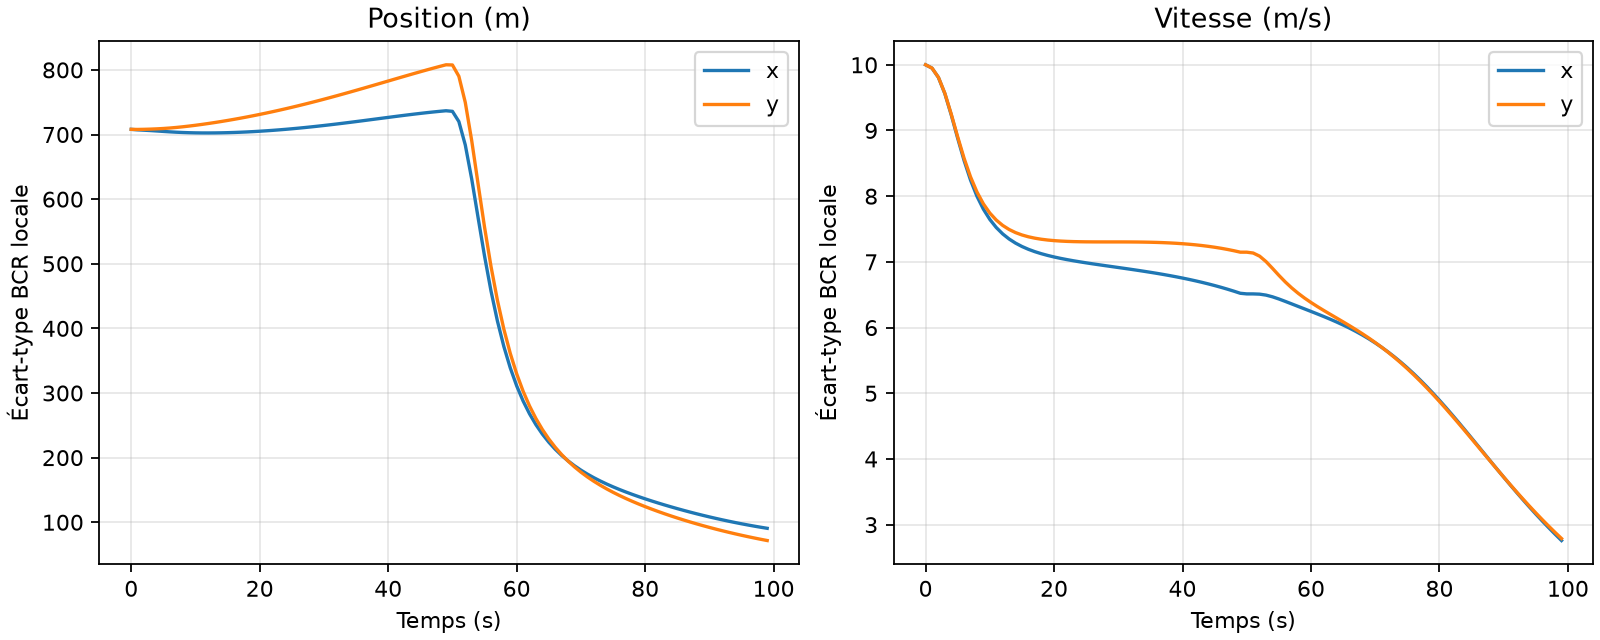
\includegraphics[width=\textwidth]{q1_incertitudes.png}
    \caption{Évolution temporelle des écarts-types associés à la BCR locale pour la position et la vitesse.}
    \label{fig:q1_incertitudes}
\end{figure}

On observe que les incertitudes sur les composantes de position augmentent légèrement durant la première partie de la trajectoire. Cette augmentation traduit la difficulté à déterminer précisément la position de la cible à partir de mesures angulaires lorsque l'observateur conserve son cap initial.

Au voisinage de l'instant de la manœuvre (\(t \approx 50\,\mathrm{s}\)), les incertitudes diminuent fortement. Le changement de cap modifie la géométrie d'observation et apporte ainsi une information supplémentaire sur l'état de la cible. Après la manœuvre, les incertitudes continuent globalement à diminuer jusqu'à la dernière mesure.

Les incertitudes associées aux composantes de vitesse diminuent également au cours du temps, avec une évolution qui dépend de la géométrie d'observation. Ces résultats illustrent l'intérêt de la manœuvre pour améliorer la précision du pistage.

\section{Conclusion générale}

Ce travail a permis d'étudier l'influence de la
manoeuvre de l'observateur sur la précision du
pistage d'un émetteur à partir de mesures angulaires,
en utilisant la borne de Cramèr-Rao.

L'étude du cas $\varphi=0$ sans information a priori
a mis en évidence une perte d'observabilité,
car la matrice d'information finale est singulière.
Ce résultat montre les limites du pistage lorsque
l'observateur conserve une trajectoire rectiligne.

L'optimisation numérique a ensuite permis d'identifier
un angle de manoeuvre optimal de $114.9^\circ$ pour
le scénario étudié, correspondant à une RMS finale
minimale de $115.540\,\mathrm{m}$.

Ces résultats montrent que la manoeuvre de
l'observateur joue un rôle essentiel dans
l'amélioration de l'observabilité et de la précision
du pistage par mesures angulaires.
La borne de Cramèr-Rao constitue ainsi un outil
théorique permettant de comparer les trajectoires
et d'identifier celle offrant les meilleures
performances d'estimation.


\end{document}
